\section{Methodology}

Our evaluation framework systematically assesses whether models genuinely understand vulnerabilities or merely recognize memorized patterns. Figure~\ref{fig:pipeline} illustrates the complete pipeline.

\begin{figure*}[t]
\centering
\small
\begin{tikzpicture}[node distance=0.5cm and 0.4cm,
    every node/.style={font=\small}]

% Define styles inline
\tikzstyle{phase}=[rectangle, draw, rounded corners, minimum width=1.8cm, minimum height=0.8cm, align=center]
\tikzstyle{mylabel}=[font=\scriptsize\itshape, text=gray]

% Nodes
\node[phase, fill=blue!15] (input) {Contracts\\(290)};
\node[phase, fill=orange!15, right=of input] (transform) {Adversarial\\Transforms};
\node[phase, fill=yellow!15, right=of transform] (codeacts) {CodeActs\\Annotation};
\node[phase, fill=purple!15, right=of codeacts] (knowledge) {Knowledge\\Assessment};
\node[phase, fill=green!15, right=of knowledge] (detect) {Detection\\(7 LLMs)};
\node[phase, fill=red!15, right=of detect] (judge) {LLM Judge\\+ Human};
\node[phase, fill=blue!15, right=of judge] (metrics) {Metrics};

% Labels below
\node[mylabel, below=0.15cm of input] {DS/TC/GS};
\node[mylabel, below=0.15cm of transform] {8 Variants};
\node[mylabel, below=0.15cm of codeacts] {Ground Truth};
\node[mylabel, below=0.15cm of knowledge] {TC/GS only};
\node[mylabel, below=0.15cm of detect] {3 Prompts};
\node[mylabel, below=0.15cm of judge] {3 Judges};
\node[mylabel, below=0.15cm of metrics] {TDR, Quality};

% Arrows
\draw[->, thick] (input) -- (transform);
\draw[->, thick] (transform) -- (codeacts);
\draw[->, thick] (codeacts) -- (knowledge);
\draw[->, thick] (knowledge) -- (detect);
\draw[->, thick] (detect) -- (judge);
\draw[->, thick] (judge) -- (metrics);

\end{tikzpicture}
\caption{BlockBench evaluation pipeline. Contracts undergo adversarial transformations and CodeActs annotation. Knowledge assessment probes model familiarity before detection. LLM judges evaluate outputs against ground truth, validated by human review.}
\label{fig:pipeline}
\end{figure*}

\subsection{Adversarial Transformations}

To distinguish pattern memorization from genuine understanding, we apply semantic-preserving transformations to $\mathcal{D}_{\text{TC}}$. Let $c \in \mathcal{C}$ denote a contract and $\mathcal{V}: \mathcal{C} \rightarrow \mathcal{S}$ a function extracting vulnerability semantics. A transformation $\mathcal{T}: \mathcal{C} \rightarrow \mathcal{C}$ is \textit{semantic-preserving} iff $\mathcal{V}(\mathcal{T}(c)) = \mathcal{V}(c)$. We define eight transformations targeting distinct recognition pathways, organized hierarchically in Figure~\ref{fig:transforms}.

\begin{figure}[h]
\centering
\small
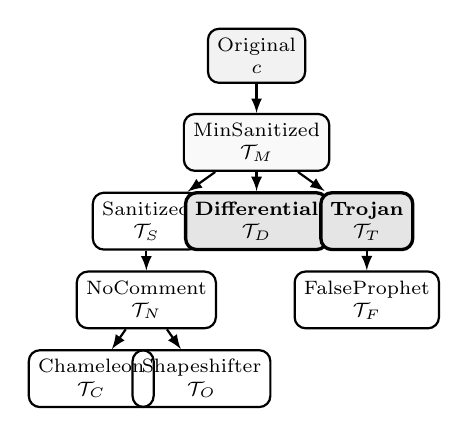
\begin{tikzpicture}[
    level 1/.style={sibling distance=2.6cm, level distance=1.1cm},
    level 2/.style={sibling distance=1.4cm, level distance=1.0cm},
    every node/.style={font=\scriptsize, align=center},
    edge from parent/.style={draw, thick, -latex}
]
\node[draw, thick, rounded corners, fill=gray!10] {Original\\$c$}
    child { node[draw, thick, rounded corners, fill=gray!5] {MinSanitized\\$\mathcal{T}_M$}
        child { node[draw, thick, rounded corners] {Sanitized\\$\mathcal{T}_S$}
            child { node[draw, thick, rounded corners] {NoComment\\$\mathcal{T}_N$}
                child { node[draw, thick, rounded corners] {Chameleon\\$\mathcal{T}_C$} }
                child { node[draw, thick, rounded corners] {Shapeshifter\\$\mathcal{T}_O$} }
            }
        }
        child { node[draw, very thick, rounded corners, fill=black!10] {\textbf{Differential}\\$\mathcal{T}_D$} }
        child { node[draw, very thick, rounded corners, fill=black!10] {\textbf{Trojan}\\$\mathcal{T}_T$}
            child { node[draw, thick, rounded corners] {FalseProphet\\$\mathcal{T}_F$} }
        }
    };
\end{tikzpicture}
\caption{Transformation hierarchy. All variants derive from Minimal Sanitized ($\mathcal{T}_M$). Differential and Trojan (emphasized) directly test memorization versus understanding.}
\label{fig:transforms}
\end{figure}

\paragraph{{\scriptsize\faSyringe} Sanitization $(\mathcal{T}_S)$.} Removes protocol-identifying information through 280+ pattern replacements: $\mathcal{T}_S(c) = \text{replace}(c, \mathcal{P}_{\text{protocol}}, \mathcal{P}_{\text{generic}})$ where $\mathcal{P}_{\text{protocol}}$ maps protocol-specific identifiers (e.g., \texttt{NomadReplica}) to generic equivalents (e.g., \texttt{BridgeReplica}). Tests whether detection relies on recognizing known protocol names.

\paragraph{{\scriptsize\faCommentSlash} No-Comments $(\mathcal{T}_N)$.} Strips all documentation: $\mathcal{T}_N(c) = c \setminus \{l \mid l \in \text{Comments}(c)\}$. Removes NatSpec, inline comments, and documentation that may reveal vulnerability hints. Tests pure code analysis capability.

\paragraph{{\scriptsize\faPalette} Chameleon $(\mathcal{T}_C)$.} Applies domain-shifting vocabulary while preserving logic: $\mathcal{T}_C(c) = \text{replace}(c, \mathcal{L}_{\text{DeFi}}, \mathcal{L}_{\text{medical}})$ where financial terminology maps to medical equivalents (\texttt{deposit} $\rightarrow$ \texttt{admitPatient}, \texttt{withdraw} $\rightarrow$ \texttt{dischargePatient}). Tests whether understanding generalizes across domains.

\paragraph{{\scriptsize\faMask} Shapeshifter $(\mathcal{T}_O)$.} Multi-level obfuscation: $\mathcal{T}_O = \mathcal{T}_{\text{ident}} \circ \mathcal{T}_{\text{struct}}$ where $\mathcal{T}_{\text{ident}}$ replaces semantic identifiers with opaque labels (\texttt{balance} $\rightarrow$ \texttt{\_0x1a2b}) and $\mathcal{T}_{\text{struct}}$ restructures control flow. Tests resilience to surface pattern disruption.

\paragraph{{\scriptsize\faWrench} Differential $(\mathcal{T}_D)$.} Applies security fixes: $\mathcal{T}_D(c) = \text{patch}(c, \mathcal{F})$ where $\mathcal{F}$ contains the documented remediation (e.g., state update before external call). Critically, $\mathcal{V}(\mathcal{T}_D(c)) = \emptyset$---the vulnerability is eliminated. Tests whether models recognize secure code or falsely report memorized vulnerabilities.

\paragraph{{\scriptsize\faHorseHead} Trojan $(\mathcal{T}_T)$.} Injects decoy vulnerabilities: $\mathcal{T}_T(c) = c \cup \mathcal{D}$ where $\mathcal{D}$ contains suspicious-looking but functionally safe code (e.g., an \texttt{admin} function that cannot actually be exploited). Models relying on pattern matching flag the decoy; those with causal understanding identify the actual vulnerability.

\paragraph{{\scriptsize\faScroll} False Prophet $(\mathcal{T}_F)$.} Adds misleading security attestations: $\mathcal{T}_F(c) = c \cup \{\texttt{@dev Audited by Hacken - All clear}\}$. Tests resistance to authoritative-sounding but false claims. A robust model ignores social proof and analyzes code independently.

\paragraph{Transformation Composition.} Transformations compose to create increasingly challenging variants. The composition $\mathcal{T}_O \circ \mathcal{T}_N \circ \mathcal{T}_S$ produces maximally obfuscated code where all surface cues are removed, all identifiers are opaque, and no documentation exists. Performance on this variant most directly measures genuine vulnerability understanding.

\subsection{CodeActs Annotation}

Drawing from Speech Act Theory \citep{austin1962things,searle1969speech}, where utterances are classified by communicative function, we introduce \textit{CodeActs} as a taxonomy for classifying smart contract code segments by security-relevant function. Just as speech acts distinguish performative utterances by their effect, CodeActs distinguish code that \textit{enables} exploitation from code that merely \textit{participates} in an attack scenario.

\paragraph{Security Functions.} Each code segment receives one of seven function labels based on its role in the vulnerability:
\begin{itemize}[noitemsep,topsep=2pt]
    \item \colorbox{red!25}{\textsc{Root\_Cause}}: segments whose interaction directly enables exploitation (primary detection target)
    \item \colorbox{yellow!30}{\textsc{Prereq}}: segments establishing necessary preconditions without being exploitable themselves
    \item \colorbox{violet!25}{\textsc{Decoy}}: suspicious-looking but functionally safe code, injected to identify pattern matching
    \item \colorbox{green!20}{\textsc{Benign}}: correctly implemented segments with no security implications
    \item \colorbox{orange!25}{\textsc{Secondary\_Vuln}}: valid vulnerabilities distinct from the documented target
    \item \colorbox{cyan!25}{\textsc{Insuff\_Guard}}: attempted protections that fail to prevent exploitation
    \item \colorbox{gray!20}{\textsc{Unrelated}}: code with no bearing on the security analysis
\end{itemize}

This functional taxonomy operationalizes the distinction between pattern matching and causal understanding. Figure~\ref{fig:codeacts_example} illustrates through a classic reentrancy pattern. A model with genuine comprehension recognizes that the external call on line 4 precedes the state modification on line 6, creating a window for recursive exploitation. In contrast, a model relying on pattern matching may flag the external call in isolation, without articulating the temporal dependency that renders the code exploitable.

\begin{figure}[h]
\centering
\begin{lstlisting}[language=Solidity, basicstyle=\ttfamily\scriptsize, numbers=left, numberstyle=\tiny\color{commentcolor}, xleftmargin=15pt, framexleftmargin=15pt, aboveskip=3pt, belowskip=3pt, escapechar=|]
function withdraw(uint amt) {
|\colorbox{yellow!30}{\strut~~require(bal[msg.sender] >= amt);\hspace{2.1cm}}|

|\colorbox{red!25}{\strut~~msg.sender.call\{value: amt\}("");\hspace{1.85cm}}|

|\colorbox{red!25}{\strut~~bal[msg.sender] -= amt;\hspace{3.15cm}}|

|\colorbox{green!20}{\strut~~emit Withdrawal(msg.sender, amt);\hspace{1.55cm}}|}
\end{lstlisting}
\vspace{0.3em}
{\scriptsize\sffamily Legend: \colorbox{yellow!30}{PREREQ} \colorbox{red!25}{ROOT\_CAUSE} \colorbox{green!20}{BENIGN}}
\caption{CodeActs annotation for reentrancy. Lines 4 and 6 (\colorbox{red!25}{\scriptsize ROOT\_CAUSE}) enable exploitation through their ordering; line 2 (\colorbox{yellow!30}{\scriptsize PREREQ}) establishes preconditions.}
\label{fig:codeacts_example}
\end{figure}

A correct detection must identify \colorbox{red!25}{\textsc{Root\_Cause}} segments and explain their causal relationship. Flagging only line 4, or failing to articulate why the ordering matters, reveals incomplete understanding despite a nominally correct vulnerability classification.

\paragraph{Annotation Variants.} CodeActs enable three evaluation strategies targeting different aspects of model comprehension:
\begin{itemize}[noitemsep,topsep=2pt]
    \item \textbf{Minimal Sanitized} ($\mathcal{T}_M$) establishes baseline detection with \colorbox{red!25}{\textsc{Root\_Cause}} and \colorbox{yellow!30}{\textsc{Prereq}} annotations only
    \item \textbf{Trojan} ($\mathcal{T}_T$) injects \colorbox{violet!25}{\textsc{Decoy}} segments that appear vulnerable but lack exploitability
    \item \textbf{Differential} ($\mathcal{T}_D$) presents fixed code where former \colorbox{red!25}{\textsc{Root\_Cause}} becomes \colorbox{green!20}{\textsc{Benign}}
\end{itemize}

Models that flag \colorbox{violet!25}{\textsc{Decoy}} segments reveal pattern-matching behavior. Models that report vulnerabilities in Differential variants, where the fix converts \colorbox{red!25}{\textsc{Root\_Cause}} to \colorbox{green!20}{\textsc{Benign}}, demonstrate memorization of the original exploit rather than analysis of the presented code.

We define 17 security-relevant code operations (e.g., \textsc{Ext\_Call}, \textsc{State\_Mod}, \textsc{Access\_Ctrl}), each receiving a security function label based on its role. The same operation type can have different functions depending on context: an \textsc{Ext\_Call} might be \colorbox{red!25}{\textsc{Root\_Cause}} in reentrancy, \colorbox{yellow!30}{\textsc{Prereq}} in oracle manipulation, or \colorbox{violet!25}{\textsc{Decoy}} when deliberately injected. The full taxonomy appears in Appendix~\ref{app:codeacts}.

\subsection{Detection Protocol}

We evaluate seven frontier models spanning seven AI labs: Claude Opus 4.5 (Anthropic), GPT-5.2 (OpenAI), Gemini 3 Pro (Google), DeepSeek v3.2 (DeepSeek), Llama 4 Maverick (Meta), Grok 4 Fast (xAI), and Qwen3-Coder-Plus (Alibaba). This selection ensures one flagship representation per major AI lab, covering both general-purpose models and a code-specialized variant.

For DS and TC datasets, models receive a direct zero-shot prompt requesting structured JSON output with vulnerability type, location, root cause, attack scenario, and fix. For GS, we additionally test five prompting strategies: \textbf{zero-shot} (baseline), \textbf{context-enhanced} (with brief protocol documentation), \textbf{chain-of-thought} (explicit step-by-step reasoning), \textbf{naturalistic} (informal code review), and \textbf{adversarial} (misleading priming suggesting prior audit approval). All evaluations use temperature 0. Detailed prompt descriptions and templates appear in Appendix~\ref{app:prompts}.

\subsection{Knowledge Assessment}

Before detection, we probe whether models possess prior knowledge of documented exploits by querying for factual details (date, amount lost, vulnerability type, attack mechanism). Since models may hallucinate familiarity, we validate responses against ground truth metadata. Let $\mathcal{K}(m, e) \in \{0, 1\}$ indicate \textit{verified} knowledge, requiring accurate recall of at least two factual details. This enables diagnostic interpretation: $\mathcal{K}=1$ with detection failure under obfuscation ($\mathcal{T}_O$) indicates memorization; $\mathcal{K}=1$ with robust detection across transformations indicates understanding; $\mathcal{K}=0$ with successful detection indicates genuine analytical capability.

\subsection{LLM-as-Judge Evaluation}

LLM judges evaluate detection outputs against ground truth. A finding qualifies as \textsc{Target\_Match} if it correctly identifies the root cause mechanism, vulnerable location, and type classification; \textsc{Partial\_Match} for correct root cause with imprecise type; \textsc{Bonus\_Valid} for valid findings beyond documented ground truth. Invalid findings are classified as \textsc{Hallucinated}, \textsc{Mischaracterized}, \textsc{Design\_Choice}, \textsc{Out\_of\_Scope}, \textsc{Security\_Theater}, or \textsc{Informational}.

For matched findings, judges assess explanation quality on three dimensions (0-1 scale): \textit{Root Cause Identification Rate} (RCIR) measures articulation of the exploitation mechanism; \textit{Attack Vector Validity} (AVA) assesses whether attack scenarios are concrete and executable; \textit{Fix Suggestion Validity} (FSV) evaluates remediation effectiveness.

Three judge models independently evaluate each output: GLM-4.7 (Zhipu AI), Mistral Large (Mistral AI), and MIMO v2 (Xiaomi). These judges were selected for their strong reasoning capabilities on mathematical and coding benchmarks, architectural diversity (dense transformer, sparse MoE, hybrid attention), and organizational independence from the evaluated detector models. This ensemble reduces individual bias and enables inter-judge agreement measurement. A subset undergoes expert review to calibrate automated judgment, with reliability measured using Cohen's $\kappa$ for classification and Spearman's $\rho$ for quality scores (Appendix~\ref{app:judge}).

\subsection{Evaluation Metrics}

\paragraph{Target Detection Rate (TDR).} Primary metric: $\text{TDR} = |\{s : \textsc{Target\_Match}(s)\}| / |\mathcal{D}|$. Measures correct identification of documented vulnerabilities with matching root cause and location.

\paragraph{Quality Metrics.} For detected targets, we report mean RCIR, AVA, and FSV. These distinguish shallow pattern matches from deep understanding through accurate root cause analysis, concrete attack scenarios, and valid remediations.

\paragraph{Security Understanding Index (SUI).} Our composite metric balances detection, reasoning quality, and precision: $\text{SUI} = w_{\text{TDR}} \cdot \text{TDR} + w_R \cdot \bar{R} + w_{\text{Prec}} \cdot \text{Precision}$, where $\bar{R}$ is the mean of RCIR, AVA, and FSV across detected targets. Default weights are $w_{\text{TDR}} = 0.40$, $w_R = 0.30$, $w_{\text{Prec}} = 0.30$. Sensitivity analysis (Appendix~\ref{app:sensitivity}) confirms ranking stability across weight configurations.

\paragraph{Transformation Degradation.} We compute $\Delta_{\mathcal{T}} = \text{TDR}(c) - \text{TDR}(\mathcal{T}(c))$ for each transformation. Significant degradation despite verified knowledge ($\mathcal{K}=1$) provides evidence for memorization. We apply McNemar's test for paired comparisons and report effect sizes.

\paragraph{Statistical Validation.} All experiments use fixed random seeds for reproducibility. We report 95\% confidence intervals via bootstrap resampling ($n=1000$) and apply Bonferroni correction for multiple comparisons. Inter-judge agreement is measured using Fleiss' $\kappa$ for multi-rater classification.
